Odin lies between the user and the relational database it is built upon, introducing learning capabilities to its query optimizer. It extends the client interface provided by the database system with commands that infer the best set of strategy settings on a per-query basis.

Upon receiving a query, it evaluates different plans under different optimizer strategy settings and tries finding the configuration that results in the lowest runtime. To do so, it relies on the underlying optimizer to produce different execution plans under different configurations. It takes advantage of query plan execution information and statistics that databases systems provide (i.e., type of operators involved, the cardinality estimates, and execution cost) before execution. These are then used to construct a vectorized representation of each plan, which is later fed into a predictive model and evaluated based on its predicted outcome.

The architecture of Odin is based on three different modules: (1) the Parser and Featurizer, (2) the Learning Module, and (3) the Configuration Tuner. Figure \ref{fig:architecture} illustrates the solution's architecture and how the different modules interact with each other. Next, we describe in further detail the role of each module.

\begin{figure}[H]
\centering
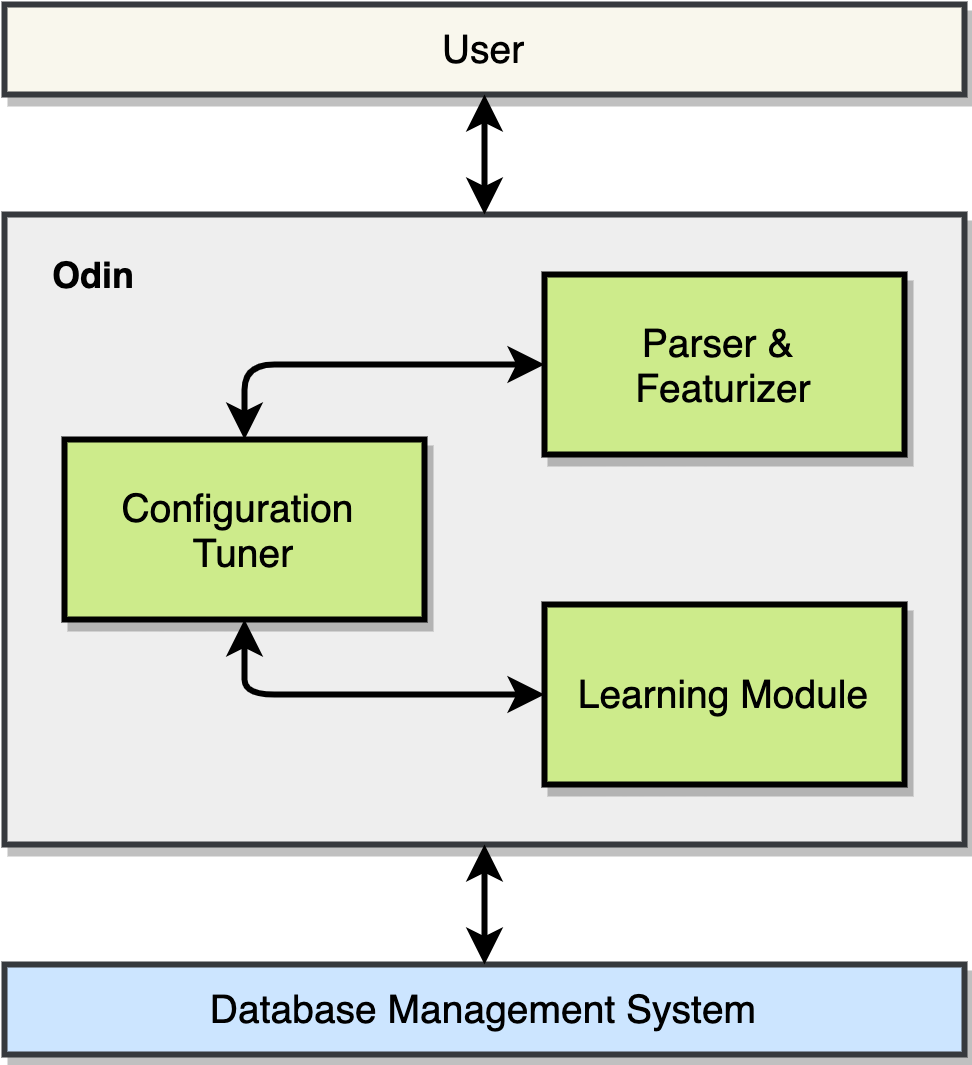
\includegraphics[width=0.5\textwidth]{img/solution/architecture.png}
\caption{Odin's architecture}
\label{fig:architecture}
\end{figure}

The \textbf{Parser and Featurizer} module contains several mechanisms for reading files that contain \gls{sql} statements and extract vector representations of query plans generated by the optimizer to be further interpreted by predictive modeling techniques.

The \textbf{Learning Module} is responsible for generating, loading, and saving several types of predictive models. The module assumes the existence of previously executed queries from which the models can be obtained and relies on the plan vector representations mentioned above and their observed runtimes.

The \textbf{Configuration Tuner} is in charge of orchestrating the communication between the two as well as enabling the selection of the best alternative optimizer configuration for a particular query. It interacts with the PostgreSQL client interface to enable or disable a set of strategies based on a direct comparison between different configurations and their expected runtime, as predicted by one of the previously trained learned models.
